\chapter{Methodology}

\section{Experimental Setup (Ripes Configuration)}
The experiment utilizes the Ripes simulator to visualize instruction execution and pipeline flow. Ripes is configured as follows:
\begin{itemize}
    \item \textbf{Processor:} 5-Stage Pipelined
    \item \textbf{ISA:} RV32IM
    \item \textbf{Data Forwarding:} Default enabled
    \item \textbf{Branch Prediction:} None
\end{itemize}

\begin{figure}[h]
  \centering
  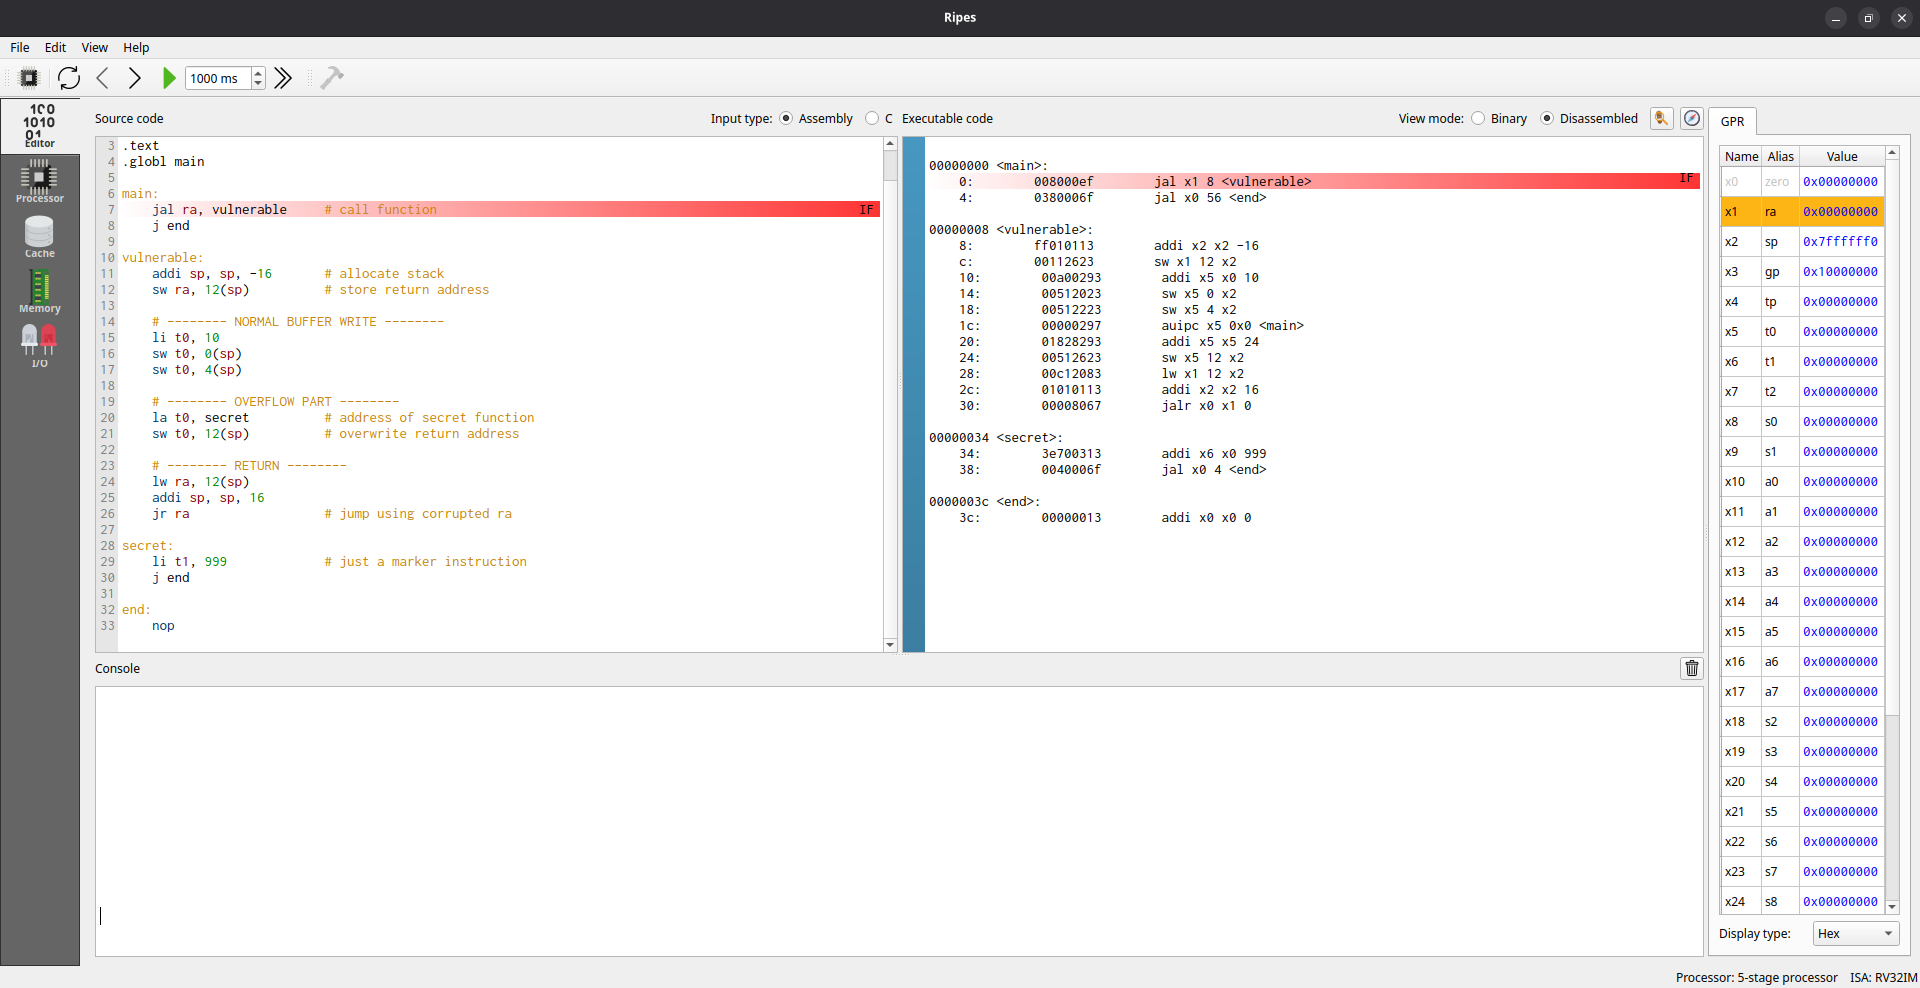
\includegraphics[width=0.8\textwidth]{images/ss1.png}
  \caption{Ripes simulator with 5-stage processor and program loaded.}
  \label{fig:ss1}
\end{figure}

\section{Program Design and Logic}
A specific RISC-V assembly program was crafted to model the attack. It contains a \texttt{main} routine, a \texttt{vulnerable} function which allocates a stack frame, and a hidden \texttt{secret} function. The complete annotated code represents the target application:

\begin{lstlisting}[language=RISCV, caption={Vulnerable RISC-V Assembly Program}]
.text
.globl main

main:
    jal ra, vulnerable      # call function; ra = addr of "j end"
    j end

vulnerable:
    addi sp, sp, -16        # allocate 16-byte stack frame
    sw ra, 12(sp)           # save legitimate return address

    # Normal buffer writes
    li t0, 10
    sw t0, 0(sp)            # buf[0] = 10
    sw t0, 4(sp)            # buf[1] = 10

    # Overflow: overwrite saved return address
    la t0, secret
    sw t0, 12(sp)           # OVERFLOW: saved ra -> address of secret

    # Return using corrupted ra
    lw ra, 12(sp)           # ra = address of secret (corrupted)
    addi sp, sp, 16
    jr ra                   # PC hijacked -> jumps to secret

secret:
    li t1, 999              # marker: proves execution reached here
    j end

end:
    nop
\end{lstlisting}

\section{Stack Memory Map}
The program allocates 16 bytes for the stack frame. The logical mapping is presented below, illustrating how the 12-byte offset creates a clear path to the return address:

\begin{table}[h]
\caption{Memory Layout within the \texttt{vulnerable} Function}
\centering
\begin{tabular}{|l|l|l|}
\hline
\textbf{Offset} & \textbf{Address (Absolute)} & \textbf{Data Purpose} \\
\hline
\texttt{sp+0} & \texttt{0x7fffffe0} & Buffer data \\
\texttt{sp+4} & \texttt{0x7fffffe4} & Buffer data \\
\texttt{sp+8} & \texttt{0x7fffffe8} & Unused \\
\texttt{sp+12} & \texttt{0x7fffffec} & Saved Return Address \\
\hline
\end{tabular}
\label{tab:methodology_stack}
\end{table}

\section{Instruction Flow Design}
The logical progression of the exploit follows six core phases based on instruction execution:
\begin{enumerate}
    \item Function setup via \texttt{jal}.
    \item Stack frame allocation and valid return address anchoring via \texttt{sw ra, 12(sp)}.
    \item Standard buffer manipulation via localized stores.
    \item The exploit trigger: a \texttt{sw} instruction explicitly targeting \texttt{12(sp)} with the address of \texttt{secret}.
    \item Corrupted context restoration via \texttt{lw ra, 12(sp)}.
    \item Control subversion via \texttt{jr ra}, violating intended control flow.
\end{enumerate}

\section{Measurement Procedure}
The procedural steps for running the test are:
\begin{enumerate}
    \item Load the compiled program into the Ripes simulator.
    \item Single-step the execution to monitor precise architectural state changes.
    \item Monitor the register panel for the value of \texttt{x1} (\texttt{ra}).
    \item Monitor the memory panel for the hex values at the dynamic stack address coordinates.
    \item Examine the pipeline diagram specifically during the execution of jump/branch instructions to identify flush conditions.
    \item Capture the architectural state at each critical instruction to record empirical evidence of the attack chain.
\end{enumerate}
